\doublespacing
\setlength{\parindent}{1cm}

\begin{flushleft}
  \textbf{Results}
\end{flushleft}

After running the fit function from the previous section, the results for the validation set came out with an accuracy of 94\% after 10 epochs. As a reminder, this result is based on the validation set that was as partition of 50 images specified by the ImageDataGenerator within Tensorflow 2.0's Keras module. This validation accuracy of 94\% tells us that this model is able to recognize 94\% of randomly selected chromagrams with labeled ragas correctly. This turns out to have a better validation accuracy than the K-Star algorithm done in previous work (Sharma and Bali, 2015) which received 93\% accuracy.

\begin{figure}
  \caption{Validation Accuracy}
  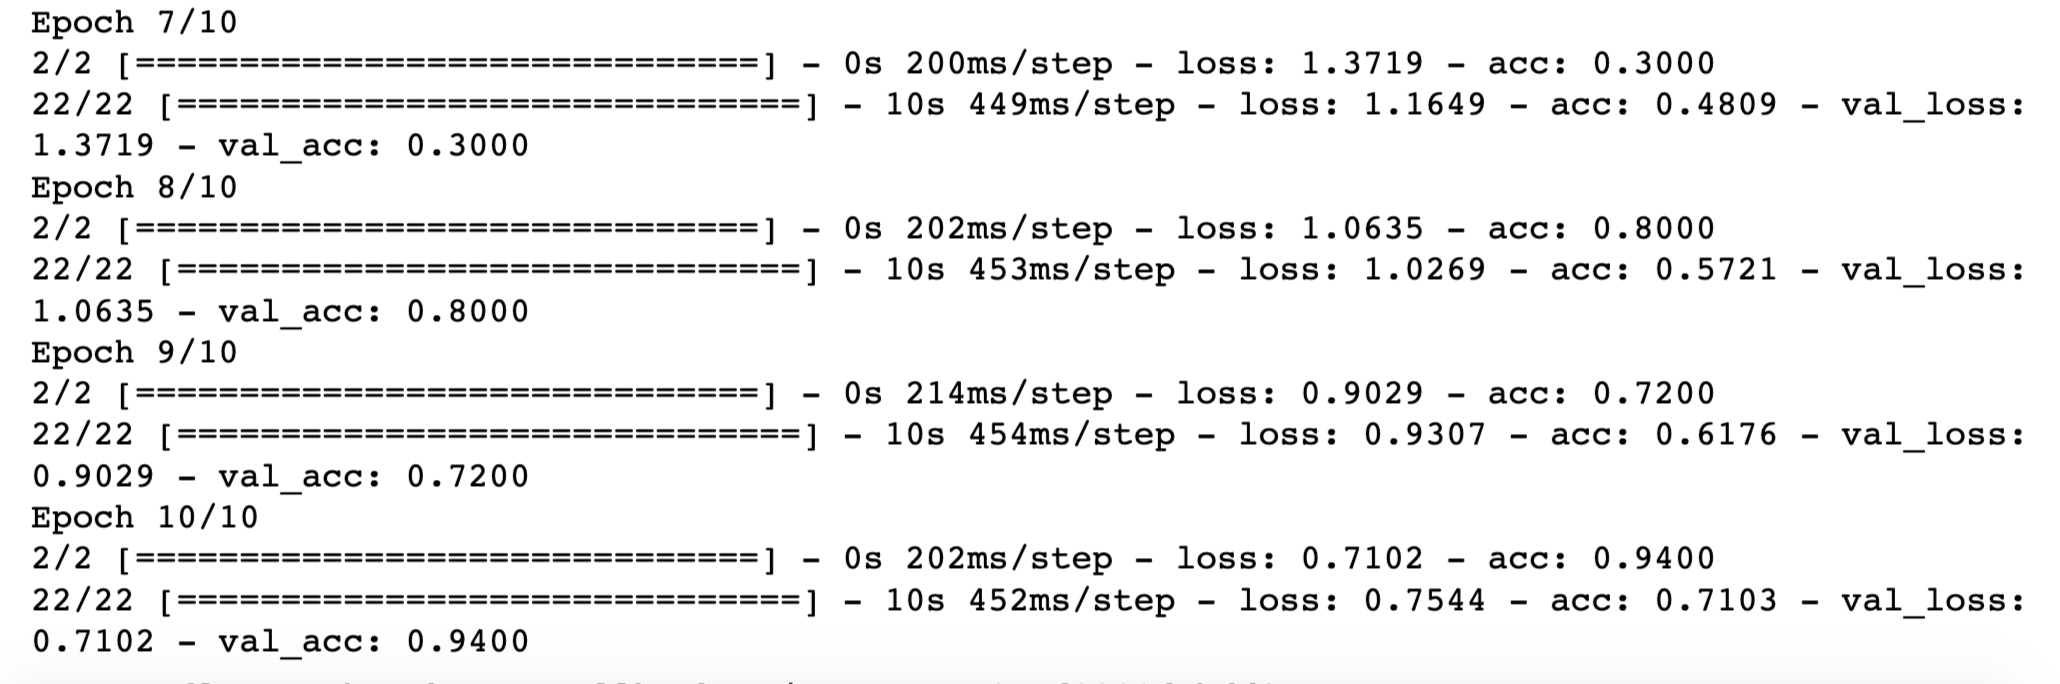
\includegraphics[width=140mm, height=50mm]{results.png}
\end{figure}

I also set aside 50 images as a hold-out test set. The test set was being used to make predictions of the raga. The results below show that the algorithm was able to correctly classify the labels of unseen data. The script for setting up this prediction is shown below as well as results.

\begin{lstlisting}
test_generator.reset()
pred=classifier.predict_generator(test_generator,
steps=STEP_SIZE_TEST,
verbose=1)

pred_bool = (pred >0.5)

predictions=[]
labels = train_generator.class_indices
labels = dict((v,k) for k,v in labels.items())
for row in pred_bool:
  l=[]
  for index,cls in enumerate(row):
      if cls:
          l.append(labels[index])
  predictions.append(",".join(l))
filenames=test_generator.filenames
results=pd.DataFrame({"file_name":filenames,
                    "predictions":predictions})
\end{lstlisting}

\begin{figure}
  \caption{Sample Prediction Table}
  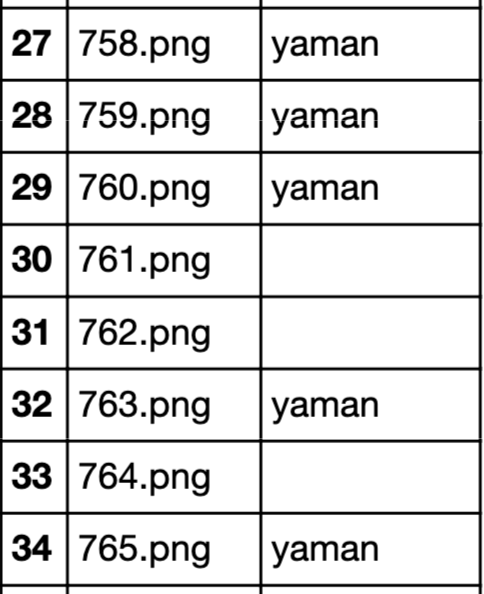
\includegraphics{pred-table.png}
\end{figure}

As seen in the above result, the CNN did not output predictions for all the samples in the test set. The reason for this is due to the pred\_bool function which has its bound specified at being greater than 0.5, but this bound is not necessarily the best number to do for multi-class classification problems.
\par
In the final chapter, I talk about my reflection on ways to improve the machine learning analysis as well as future steps for moving from a proof of concept into an intelligent raaga classification software that can be deployed into mobile applications as a tool for musicologists and composers. 
